% Add `ngerman` to documentclass for German docs
\documentclass[12pt, a4paper]{article}
\usepackage{a4wide}
\usepackage{setspace}
\usepackage{csquotes}
\usepackage[utf8]{inputenc}

\usepackage{url}
\usepackage[hidelinks]{hyperref}
\usepackage{minted}
\usemintedstyle{perldoc}

% inline code
\newcommand{\code}[1]{\texttt{#1}}

% Uncomment for German
%\usepackage[ngerman]{babel}

% For generating template dummy text
\usepackage{lipsum}

\usepackage{myColors}
\usepackage{myFooter}
\usepackage{myTitle}

% Libraries outside of template
\usepackage[T1]{fontenc}
\usepackage{upquote}
\AtBeginDocument{%
    \def\PYZsq{\textquotesingle}%
}

\usepackage{amsmath}

\usepackage{verbatim}

\usepackage{longtable}

%%%%%%%%%%%%%%%%%%%%%%%%%%%%%%%%%%%%%%%%%%%%%%%%%%%%%%%%%%%%%%%%%%%%%%%%%%%%%%%%

\project{CS 432 Web Science}
\author{Derek Goddeau}
\title{Assignment Nine}
\supervisor{Michael L. Nelson}

\doublespace
\pagestyle{hacker}

\begin{document}
\maketitle

\newpage



%%%%%%%%%%%%%%%%%%%%%%%%%%%
% Get classificaiton data %
%%%%%%%%%%%%%%%%%%%%%%%%%%%
\section{Get the blog and classification data}
 
To get the feed data I used a slightly modified version of the code from assignment eight, only changing it to save the blog entry data instead of entire blogs and to save the XML data. I used the blog \href{http://dailyvim.blogspot.com/}{Daily Vim} and the categories admin, commands, off-topic, plugins, mappings, and vimrc. I used YAML format to store the category data by title key and category since it is very friendly for human editing and can easily be loaded into a dictionary.

\section{Train the Fisher classifier and run it 50/50}

To get the data I wrote a program that deletes the database each run, and runs the classifier. I read all the data into a dictionary including the category data.

\begin{minipage}{\linewidth} % prevent splitting between pages
\vspace{2em}
\begin{minted}[fontfamily=tt]{python}
for xml in xml_files:
    feed_dict = feedparser.parse(xml)
    for entry in feed_dict['entries']:
        uri = entry.link
        title = entry.title
        content = entry.summary
        category = categories[title]
        data[uri] = {'title': title,
                     'content': content,
                     'category': category}
\end{minted}
\vspace{2em}
\end{minipage}

\newpage
Then I use a library I wrote for another project for dictionary manipulation, and slightly modified to split the dictionary into the desired parts. The library is in \href{https://github.com/hylang/hy}{hy} \code{(think (+ Python LISP))}. Hylang is a Python host language that is a LISP dialect just like Clojure is to Java, but hylang is completely bidirectional. Any hy module can be imported in any Python program and any Python program can be imported in any hy program. The dictionary split function:

\begin{minipage}{\linewidth} % prevent splitting between pages
\vspace{2em}
\begin{minted}[fontfamily=tt]{clojure}
(defn split [dictionary &optional [training 0.90]]
  "Split a dictionary by percentage"
  (setv i (iter (.items dictionary)))
  (setv d1 (dict (islice i (int (* (len (.keys dictionary)) training)))))
  (setv d2 (dict i))
  (, d1 d2))
\end{minted}
\vspace{2em}
\end{minipage}

Then I just call \code{train()} function from the PCI code over the results, and then \code{classify()} over the rest. I build actual and predcted parallel lists which are used with the \code{pandas\_ml} library \code{ConfustionMatrix} to get detailed statistics and also create the graph shown in figure~\ref{fig:5050} on page~\pageref{fig:5050}. The table showing the complete data about the predictions is in the section at the end of the document for statistics on page~\pageref{sec:5050}. Table~\ref{tab:5050} on page~\pageref{tab:5050} provides a statistics summary and the complete statistics can be viewed on page~\pageref{5050stats}.

\begin{figure}[H]
    \label{fig:5050}
    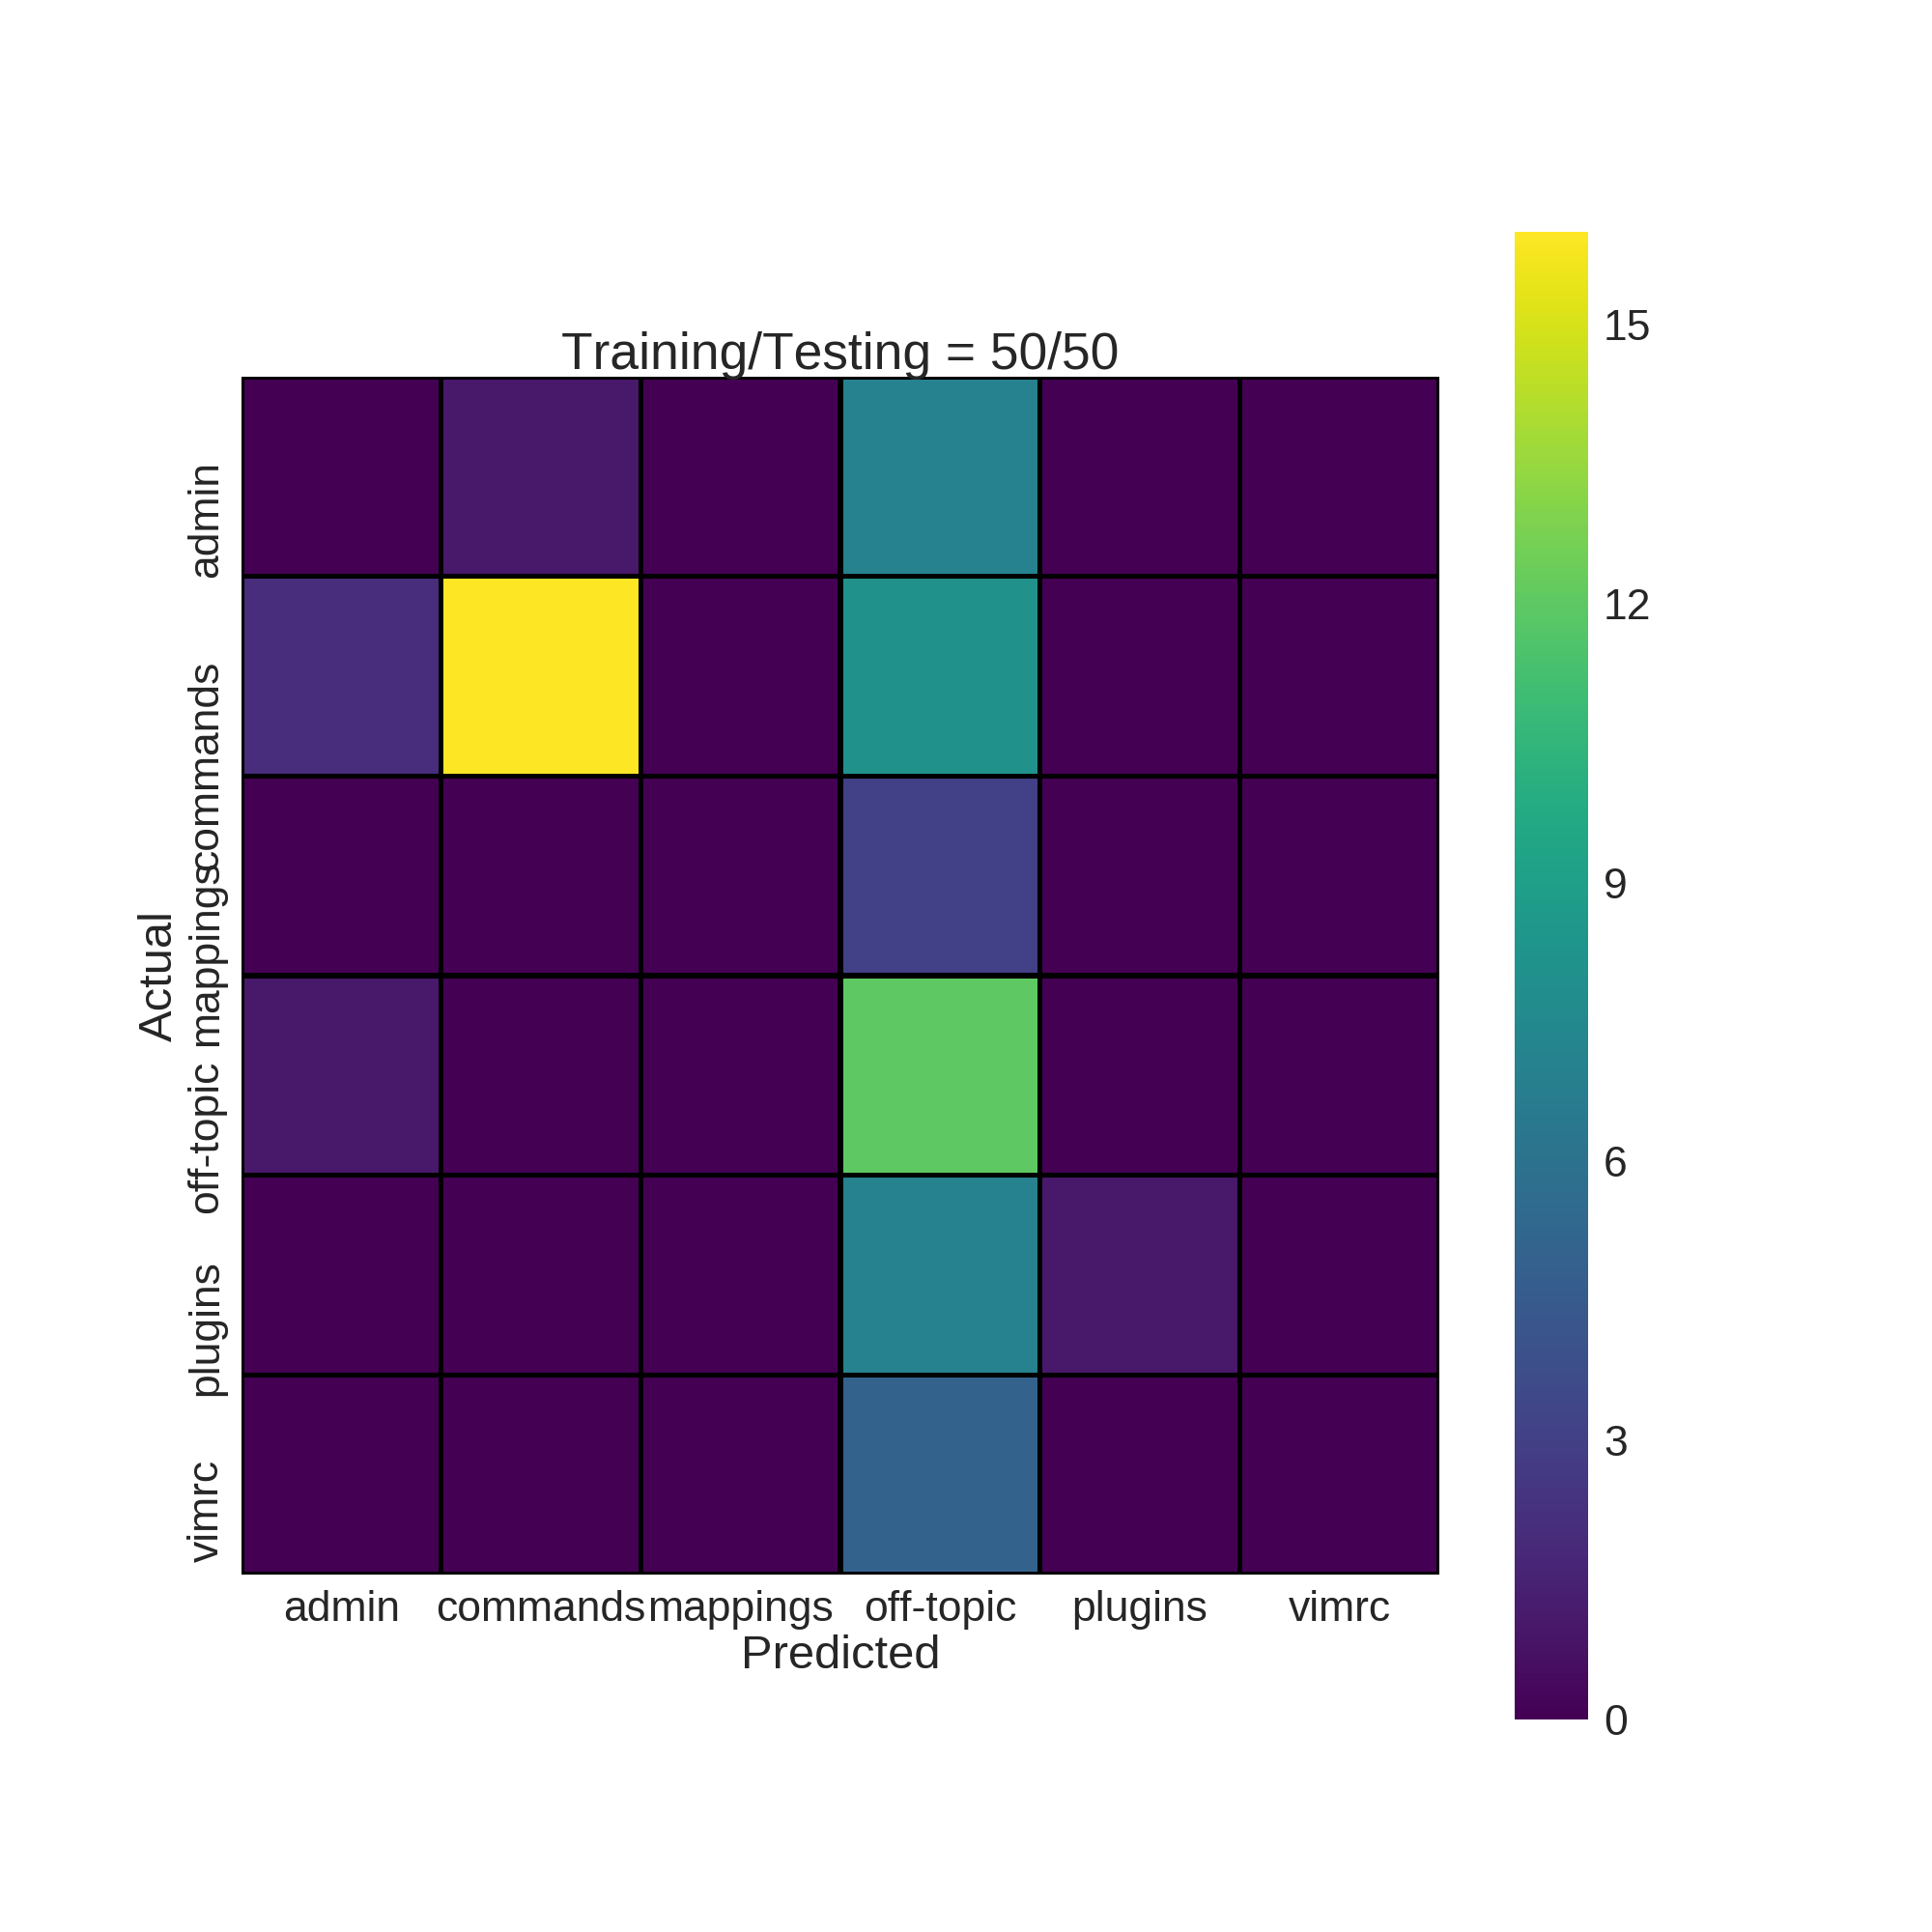
\includegraphics[width=\textwidth]{../train_validate/heatmaps/50_50.png}
\end{figure}

\begin{table}[H]
    \centering
    \label{tab:5050}
    \begin{tabular}{llll}
    \hline
    Category    & F-Measure & Precision & Recall    \\
    \hline
    admin       & 0.000     & 0.000     & 0.000     \\
    commands    & 0.783     & 0.941     & 0.615     \\
    mappings    & 0.000     & 0.000     & NaN       \\
    off-topic   & 0.436     & 0.286     & 0.923     \\
    plugins     & 0.222     & 1.000     & 0.125     \\
    vimrc       & 0.000     & NaN       & 0.000     \\
    average     & 0.240     & 0.371     & 0.277     \\
    \hline
    \end{tabular}
\end{table}

\newpage
\section{Train the Fisher classifier and run it 90/10}

For this question the exact same procedure was followed except when calling the \code{split} function I pass \code{training=0.9} instead of \code{training=0.5}. The confusion matrix results are shown below. The table showing the complete data about the predictions is in the section at the end of the document for statistics on page~\pageref{sec:9090}. Table~\ref{tab:9090} on page~\pageref{tab:9090} provides a statistics summary and the complete statistics can be viewed on page~\pageref{9090stats}.


\begin{figure}[H]
    \label{fig:9090}
    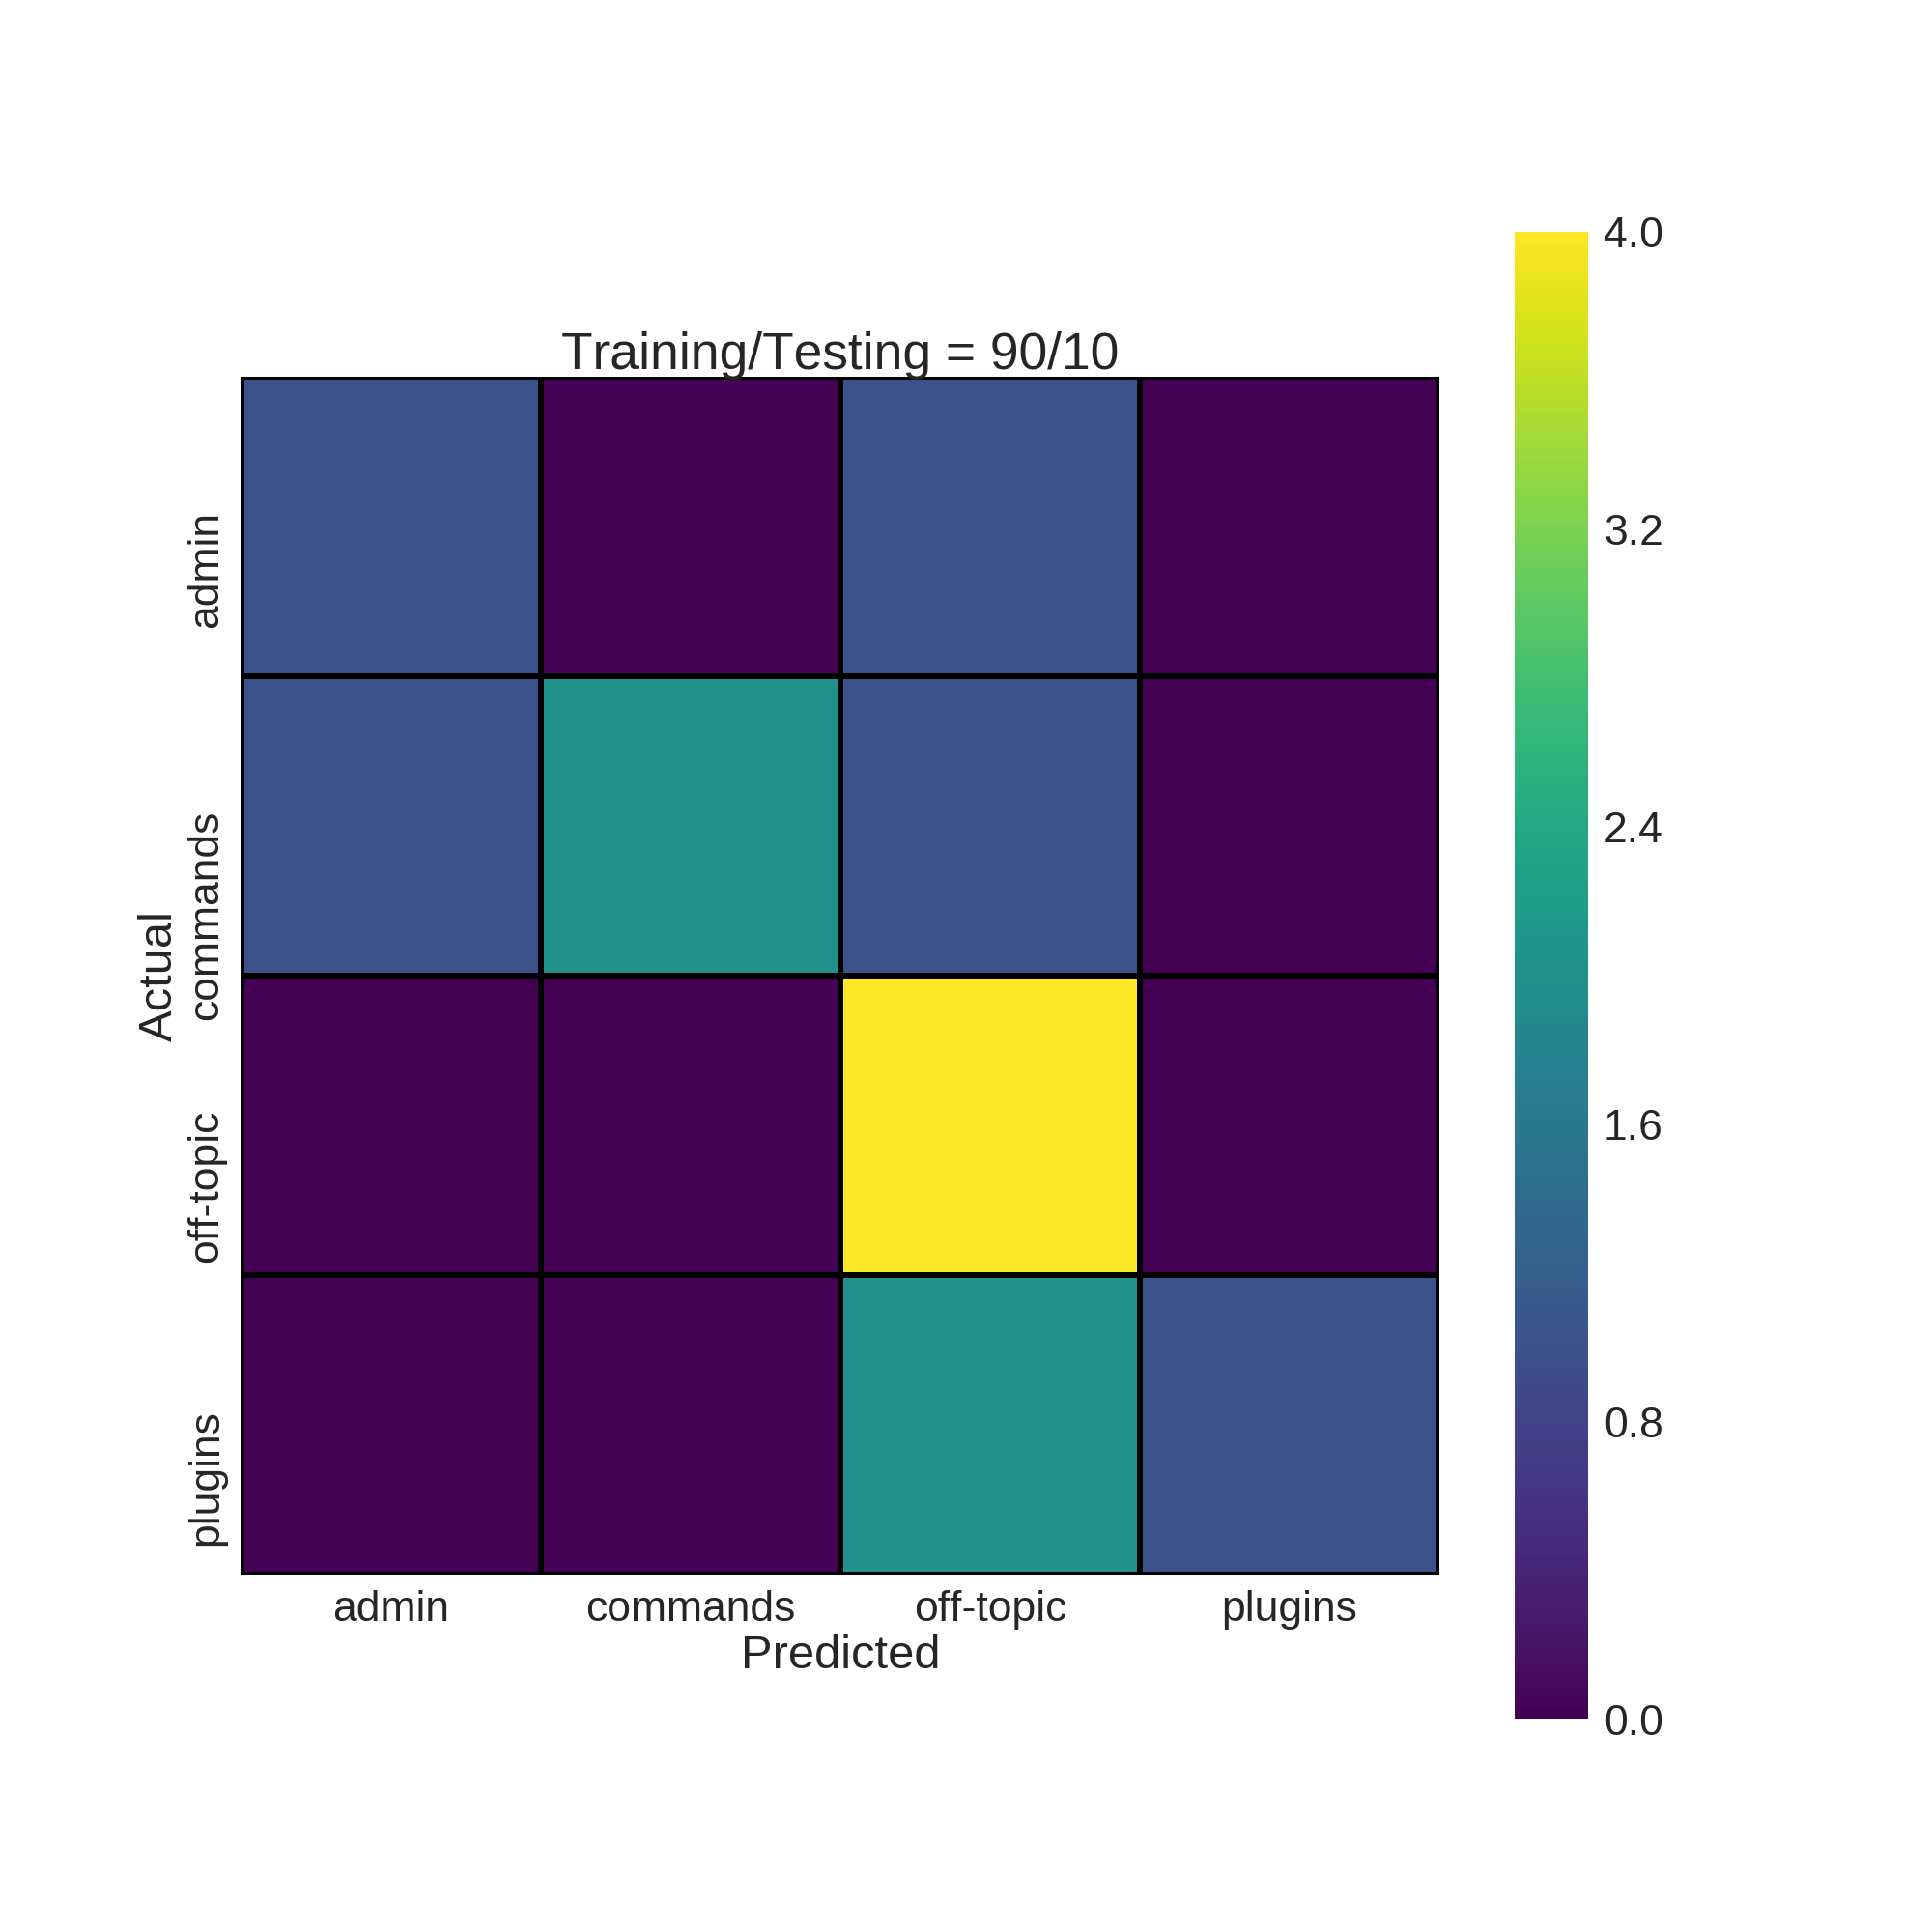
\includegraphics[width=\textwidth]{../train_validate/heatmaps/90_10.png}
\end{figure}

\begin{table}[H]
    \centering
    \label{tab:5050}
    \begin{tabular}{llll}
    \hline
    Category    & F-Measure & Precision & Recall    \\
    \hline
    admin       & 0.500     & 0.500     & 0.500     \\
    commands    & 0.667     & 1.000     & 0.500     \\
    off-topic   & 0.667     & 0.500     & 1.000     \\
    plugins     & 0.500     & 1.000     & 0.333     \\
    average     & 0.584     & 0.750     & 0.583     \\
    \hline
    \end{tabular}
\end{table}

The performance of the classifier basically doubled using this method.

\newpage
\section{data}

\label{sec:5050}
\subsection{Results from 50/50}

\subsubsection{50/50 Detailed Outcomes}
\begin{longtable}{lll}
\hline
 Title                                       & Predicted   & Actual    \\
\hline
 Pull Into Ex                                & commands    & commands  \\
 Last Insert                                 & commands    & commands  \\
 Vimperator                                  & off-topic   & plugins   \\
 Last Command                                & off-topic   & admin     \\
 Command on All Windows                      & off-topic   & commands  \\
 Share a Screen Session                      & off-topic   & admin     \\
 Vim.js                                      & off-topic   & plugins   \\
 Shift-Tab'ing                               & off-topic   & mappings  \\
 Search Register                             & commands    & commands  \\
 Vimgrep Without Object Names                & off-topic   & commands  \\
 Extending History                           & off-topic   & vimrc     \\
 Last Changed Text                           & commands    & commands  \\
 Using a Mapleader                           & off-topic   & mappings  \\
 Vim + Eclipse = Eclim                       & off-topic   & off-topic \\
 Text States                                 & off-topic   & commands  \\
 Finding and Replacing Unicode Characters    & commands    & admin     \\
 Jumping to a Buffer                         & commands    & commands  \\
 The Tao of Programming                      & off-topic   & off-topic \\
 Tabs                                        & off-topic   & mappings  \\
 The Wonderful "F" Key                       & commands    & commands  \\
 Scrollbind                                  & off-topic   & vimrc     \\
 Generating Mock Userdata                    & admin       & off-topic \\
 Vim Gitgutter                               & off-topic   & plugins   \\
 Reformat a Paragraph                        & off-topic   & commands  \\
 Modelines                                   & off-topic   & vimrc     \\
 Repeat Last Substitution                    & commands    & commands  \\
 Removing Lines that Don't Match a Pattern   & admin       & commands  \\
 Supertab                                    & off-topic   & plugins   \\
 Knowing Where You Are                       & commands    & commands  \\
 Switching from Horizontal to Vertical Split & commands    & commands  \\
 Quick Exits                                 & commands    & commands  \\
 Set  Hidden                                 & off-topic   & vimrc     \\
 Autocommands                                & off-topic   & vimrc     \\
 Question: Browsing Remote Filesystems       & off-topic   & plugins   \\
 Ubuntu Audio Sharing                        & off-topic   & off-topic \\
 PHP: Invoking a method with Map             & off-topic   & off-topic \\
 Yank S-Exp                                  & commands    & commands  \\
 bashreduce                                  & off-topic   & admin     \\
 Determining Linux Version                   & off-topic   & admin     \\
 Removing Ctrl-M                             & off-topic   & commands  \\
 Snippit Support                             & off-topic   & plugins   \\
 Indent From Normal Mode                     & commands    & commands  \\
 Twistem.FM                                  & off-topic   & off-topic \\
 Gnome Terminal Tips                         & off-topic   & admin     \\
 Types of Registers                          & off-topic   & commands  \\
 Screen in OS X Leopard                      & off-topic   & admin     \\
 Value Under Cursor \#2                       & commands    & commands  \\
 Goodbye Daily Vim, Hello Emacs              & off-topic   & off-topic \\
 Got a Question?                             & off-topic   & off-topic \\
 Vi Mode in Readline Applications            & off-topic   & commands  \\
 Unhighlight Current Search                  & commands    & commands  \\
 Vim Cookbook                                & off-topic   & off-topic \\
 Right = Left                                & admin       & commands  \\
 Sensible Defaults with Vim-Sensible         & plugins     & plugins   \\
 Snipmate                                    & off-topic   & plugins   \\
 Why Functional Programming Matters          & off-topic   & off-topic \\
 Count Words                                 & commands    & commands  \\
 Swap Characters                             & commands    & commands  \\
 Recursively Replace Ctrl-M                  & off-topic   & admin     \\
 An Introduction to Clojure's Agents         & off-topic   & off-topic \\
 Reload VIMRC                                & off-topic   & commands  \\
 Only RSS Vim Tips                           & off-topic   & off-topic \\
 The Golden Rules of Recursion               & off-topic   & off-topic \\
\hline
\end{longtable}

\newpage
\subsubsection{50/50 Detailed Stats}
\label{5050stats}
\begin{verbatim}
Predicted  admin  commands  mappings  off-topic  plugins  vimrc  __all__
Actual                                                                  
admin          0         1         0          7        0      0        8
commands       2        16         0          8        0      0       26
mappings       0         0         0          3        0      0        3
off-topic      1         0         0         12        0      0       13
plugins        0         0         0          7        1      0        8
vimrc          0         0         0          5        0      0        5
__all__        3        17         0         42        1      0       63

Classes                                    admin   commands  mappings  \
Population                                    63         63        63   
P: Condition positive                          8         26         3   
N: Condition negative                         55         37        60   
Test outcome positive                          3         17         0   
Test outcome negative                         60         46        63   
TP: True Positive                              0         16         0   
TN: True Negative                             52         36        60   
FP: False Positive                             3          1         0   
FN: False Negative                             8         10         3   
TPR: (Sensitivity, hit rate, recall)           0   0.615385         0   
TNR=SPC: (Specificity)                  0.945455   0.972973         1   
PPV: Pos Pred Value (Precision)                0   0.941176       NaN   
NPV: Neg Pred Value                     0.866667   0.782609  0.952381   
FPR: False-out                         0.0545455   0.027027         0   
FDR: False Discovery Rate                      1  0.0588235       NaN   
FNR: Miss Rate                                 1   0.384615         1   
ACC: Accuracy                           0.825397   0.825397  0.952381   
F1 score                                       0   0.744186         0   
MCC: Matthews correlation coefficient -0.0852803   0.652568       NaN   
Informedness                          -0.0545455   0.588358         0   
Markedness                             -0.133333   0.723785       NaN   
Prevalence                              0.126984   0.412698  0.047619   
LR+: Positive likelihood ratio                 0    22.7692       NaN   
LR-: Negative likelihood ratio           1.05769   0.395299         1   
DOR: Diagnostic odds ratio                     0       57.6       NaN   
FOR: False omission rate                0.133333   0.217391  0.047619   

Classes                                off-topic   plugins      vimrc  
Population                                    63        63         63  
P: Condition positive                         13         8          5  
N: Condition negative                         50        55         58  
Test outcome positive                         42         1          0  
Test outcome negative                         21        62         63  
TP: True Positive                             12         1          0  
TN: True Negative                             20        55         58  
FP: False Positive                            30         0          0  
FN: False Negative                             1         7          5  
TPR: (Sensitivity, hit rate, recall)    0.923077     0.125          0  
TNR=SPC: (Specificity)                       0.4         1          1  
PPV: Pos Pred Value (Precision)         0.285714         1        NaN  
NPV: Neg Pred Value                     0.952381  0.887097   0.920635  
FPR: False-out                               0.6         0          0  
FDR: False Discovery Rate               0.714286         0        NaN  
FNR: Miss Rate                         0.0769231     0.875          1  
ACC: Accuracy                           0.507937  0.888889   0.920635  
F1 score                                0.436364  0.222222          0  
MCC: Matthews correlation coefficient    0.27735  0.332997        NaN  
Informedness                            0.323077     0.125          0  
Markedness                              0.238095  0.887097        NaN  
Prevalence                              0.206349  0.126984  0.0793651  
LR+: Positive likelihood ratio           1.53846       inf        NaN  
LR-: Negative likelihood ratio          0.192308     0.875          1  
DOR: Diagnostic odds ratio                     8       inf        NaN  
FOR: False omission rate                0.047619  0.112903  0.0793651  
\end{verbatim}

\newpage
\label{sec:9090}
\subsection{Results from 90/10}

\subsubsection{90/10 Detailed Outcomes}
\begin{tabular}{lll}
\hline
 Title                                    & Predicted   & Actual    \\
\hline
 Unhighlight Current Search               & commands    & commands  \\
 Vim Cookbook                             & off-topic   & off-topic \\
 Right = Left                             & admin       & commands  \\
 Sensible Defaults with Vim-Sensible      & plugins     & plugins   \\
 Reload VIMRC                             & off-topic   & commands  \\
 Finding and Replacing Unicode Characters & admin       & admin     \\
 Vim Gitgutter                            & off-topic   & plugins   \\
 Swap Characters                          & commands    & commands  \\
 Recursively Replace Ctrl-M               & off-topic   & admin     \\
 An Introduction to Clojure's Agents      & off-topic   & off-topic \\
 Snipmate                                 & off-topic   & plugins   \\
 Only RSS Vim Tips                        & off-topic   & off-topic \\
 The Golden Rules of Recursion            & off-topic   & off-topic \\
\hline
\end{tabular}

\newpage
\subsubsection{90/10 Detailed Stats}
\label{9090stats}
\begin{verbatim}
Predicted  admin  commands  mappings  off-topic  plugins  vimrc  __all__
Actual                                                                  
admin          0         1         0          7        0      0        8
commands       2        16         0          8        0      0       26
mappings       0         0         0          3        0      0        3
off-topic      1         0         0         12        0      0       13
plugins        0         0         0          7        1      0        8
vimrc          0         0         0          5        0      0        5
__all__        3        17         0         42        1      0       63

Classes                                    admin   commands  mappings  \
Population                                    63         63        63   
P: Condition positive                          8         26         3   
N: Condition negative                         55         37        60   
Test outcome positive                          3         17         0   
Test outcome negative                         60         46        63   
TP: True Positive                              0         16         0   
TN: True Negative                             52         36        60   
FP: False Positive                             3          1         0   
FN: False Negative                             8         10         3   
TPR: (Sensitivity, hit rate, recall)           0   0.615385         0   
TNR=SPC: (Specificity)                  0.945455   0.972973         1   
PPV: Pos Pred Value (Precision)                0   0.941176       NaN   
NPV: Neg Pred Value                     0.866667   0.782609  0.952381   
FPR: False-out                         0.0545455   0.027027         0   
FDR: False Discovery Rate                      1  0.0588235       NaN   
FNR: Miss Rate                                 1   0.384615         1   
ACC: Accuracy                           0.825397   0.825397  0.952381   
F1 score                                       0   0.744186         0   
MCC: Matthews correlation coefficient -0.0852803   0.652568       NaN   
Informedness                          -0.0545455   0.588358         0   
Markedness                             -0.133333   0.723785       NaN   
Prevalence                              0.126984   0.412698  0.047619   
LR+: Positive likelihood ratio                 0    22.7692       NaN   
LR-: Negative likelihood ratio           1.05769   0.395299         1   
DOR: Diagnostic odds ratio                     0       57.6       NaN   
FOR: False omission rate                0.133333   0.217391  0.047619   

Classes                                off-topic   plugins      vimrc  
Population                                    63        63         63  
P: Condition positive                         13         8          5  
N: Condition negative                         50        55         58  
Test outcome positive                         42         1          0  
Test outcome negative                         21        62         63  
TP: True Positive                             12         1          0  
TN: True Negative                             20        55         58  
FP: False Positive                            30         0          0  
FN: False Negative                             1         7          5  
TPR: (Sensitivity, hit rate, recall)    0.923077     0.125          0  
TNR=SPC: (Specificity)                       0.4         1          1  
PPV: Pos Pred Value (Precision)         0.285714         1        NaN  
NPV: Neg Pred Value                     0.952381  0.887097   0.920635  
FPR: False-out                               0.6         0          0  
FDR: False Discovery Rate               0.714286         0        NaN  
FNR: Miss Rate                         0.0769231     0.875          1  
ACC: Accuracy                           0.507937  0.888889   0.920635  
F1 score                                0.436364  0.222222          0  
MCC: Matthews correlation coefficient    0.27735  0.332997        NaN  
Informedness                            0.323077     0.125          0  
Markedness                              0.238095  0.887097        NaN  
Prevalence                              0.206349  0.126984  0.0793651  
LR+: Positive likelihood ratio           1.53846       inf        NaN  
LR-: Negative likelihood ratio          0.192308     0.875          1  
DOR: Diagnostic odds ratio                     8       inf        NaN  
FOR: False omission rate                0.047619  0.112903  0.0793651  
\end{verbatim}

\end{document}
